%%%%%%%%%%%%%%%%%%%%%%%%%%%%%%%%%%%%%%%%%%%%%%%%%%%%%%%%%%%%%%%%%%%%%%%%%%%%%%%
% Titel:   Diagramm: SRF10
% Autor:   Nicola Käser
%%%%%%%%%%%%%%%%%%%%%%%%%%%%%%%%%%%%%%%%%%%%%%%%%%%%%%%%%%%%%%%%%%%%%%%%%%%%%%%
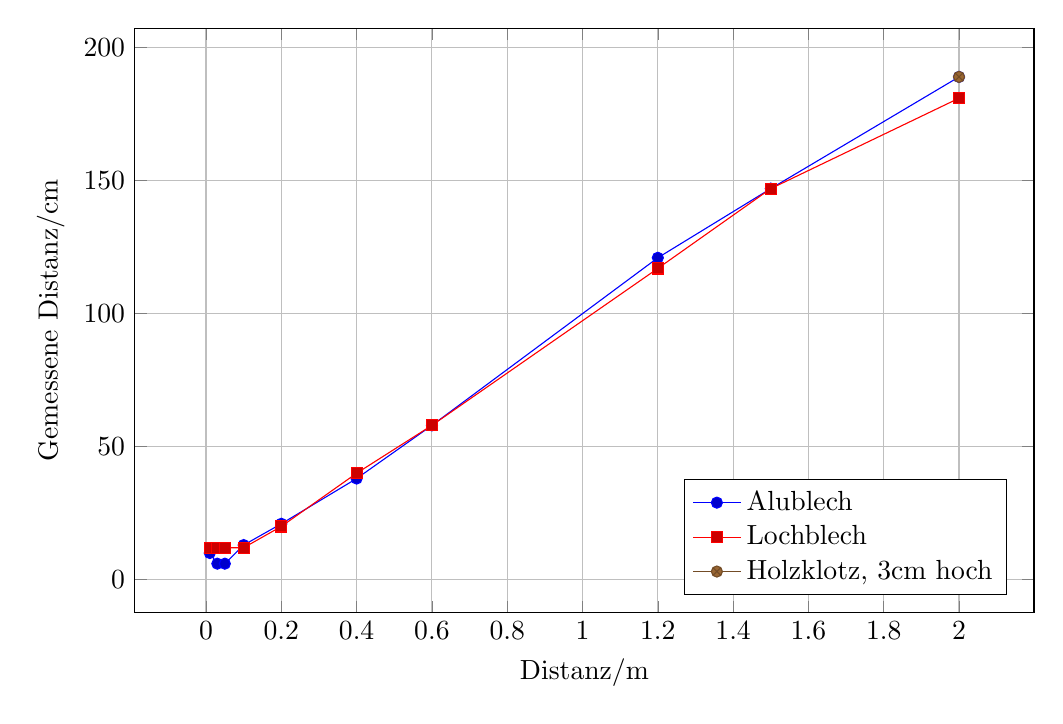
\begin{tikzpicture}
	\begin{axis}[
		height=9cm, width=13cm,
		xlabel=Distanz/m, ylabel=Gemessene Distanz/cm,
		grid=major,
		legend style={
			cells={anchor=west},
			legend pos=south east
		}]
	%
	%\addplot[color=blue,mark=*] coordinates {
	\addplot coordinates {
		(0.01,  10)
		(0.03,   6)
		(0.05,   6)
		(0.10,  13)
		(0.20,  21)
		(0.40,  38)
		(0.60,  58)
		(1.20, 121)
		(1.50, 147)
		(2.00, 189)
	};
	\addlegendentry{Alublech}
	%
	%\addplot[color=red,mark=square*] coordinates {
	\addplot coordinates {
		(0.01,  12)
		(0.03,  12)
		(0.05,  12)
		(0.10,  12)
		(0.20,  20)
		(0.40,  40)
		(0.60,  58)
		(1.20, 117)
		(1.50, 147)
		(2.00, 181)
	};
	\addlegendentry{Lochblech}
	%
	%\addplot[color=teal,mark=triangle*] coordinates {
	\addplot coordinates {
		(2, 189)
	};
	\addlegendentry{Holzklotz, 3cm hoch}
	%
	\end{axis}
\end{tikzpicture}